\documentclass[English, Lau, oneside]{sapthesis}
%\usepackage{hyperref}
\usepackage{microtype}
\usepackage[english]{babel}
\usepackage[utf8]{inputenx}
\usepackage{graphicx}
\usepackage{float} % Include the float package
\usepackage{skmath}
\usepackage{amsmath, xparse}
\usepackage{wrapfig}
\usepackage{float}
\usepackage{amsmath,amssymb}
\usepackage{sidecap}
\usepackage{xcolor}
\usepackage{gensymb}
\usepackage{caption}
\usepackage{tabularx}
\usepackage{geometry}
\usepackage[utf8]{inputenx}
\usepackage{indentfirst}
\usepackage{microtype}
\usepackage[italian]{babel}
\usepackage{siunitx}
\DeclareMathOperator\erf{erf}
\usepackage{hyperref}
\usepackage{csvsimple}
\usepackage{subfig}
\usepackage{placeins}
\usepackage{xfrac}
\usepackage[makeroom]{cancel}
\usepackage{verbatim}
\usepackage{ gensymb }
\usepackage{ longtable }
\usepackage{geometry}
\usepackage{eucal}
%\usepackage{hyperref}
\usepackage{braket}
\usepackage{bbold}
\usepackage[hidelinks]{hyperref}
\usepackage{indentfirst}
\usepackage{microtype}
\usepackage{amsmath}
\usepackage{siunitx}
\usepackage[titles]{tocloft}


%\usepackage{chemformula}
%\usepackage{setspace}
%\usepackage{yfonts,color}
%\usepackage{siunitx}
%\usepackage{comment}
%\usepackage{multirow}
%\usepackage{varioref}
%\usepackage[bottom]{footmisc}
%\usepackage{wrapfig}
%\usepackage{float}
%\usepackage{type1cm}
%\usepackage{chngcntr}
%\onehalfspacing
%\counterwithout{footnote}{chapter}
\usepackage{hyperref}
\usepackage{hyperref}
\hypersetup{
			hyperfootnotes=true,			
			bookmarks=true,			
			colorlinks=true,
			linkcolor=red,
                        linktoc=page,
			anchorcolor=black,
			citecolor=red,
			urlcolor=blue,
			pdftitle={La natura particellare della materia oscura},
			pdfauthor={Enrico Bignozzi},
			pdfkeywords={thesis, sapienza, roma, university}
 }


\hypersetup{pdftitle={Sapthesis class example},pdfauthor={Francesco Beccari}}

% Remove in a normal thesis
\usepackage{lipsum}
\usepackage{curve2e}
\definecolor{gray}{gray}{0.4}
\newcommand{\bs}{\textbackslash}

% Commands for the titlepage
\title{}
\author{}
\IDnumber{}
\course{Corso di Laurea Magistrale in Fisica}
\courseorganizer{Facoltà di Scienze Matematiche, Fisiche e Naturali}
\AcademicYear{}
\copyyear{}
\advisor{}
\coadvisor{}
\authoremail{}

%\examdate{16 April 2013}
%\examiner{Prof. Nome Cognome}
%\examiner{Prof. Nome Cognome}
%\examiner{Dr. Nome Cognome}
%\versiondate{\today}
\begin{document}
\maketitle
\tableofcontents\addcontentsline{toc}{chapter}{Indice}
\addcontentsline{toc}{chapter}{Indice}
\tableofcontents

%\begin{abstract}

%\end{abstract}

%\begin{acknowledgments}
    
%\end{acknowledgments}

\dedication{}

\newpage
\null
\thispagestyle{empty}
\newpage


% Do not use the starred version of the chapter command!


\newpage
\null
\thispagestyle{empty}
\newpage



\chapter*{Introduction}
\addcontentsline{toc}{chapter}{Introduction}
\noindent
Proteins are the constituents of life and the foundation of the functionality of living organisms . \cite{ref}
They are constituted by a sequence of amino acids, a set of atoms, that fold into a three-dimensional structure that determines their function. 
The study of proteins is crucial for understanding the molecular basis of life and for the development of new drugs.
The determination of the three-dimensional structure of a protein is a fundamental step in the study of its function.

Among the main functions of proteins are:
\begin{itemize}
    \item \textbf{Enzymatic catalysis}: Enzymatic proteins accelerate chemical reactions by reducing activation energy and regulating cellular metabolic processes.
    \item \textbf{Structural roles}: Some proteins, such as collagen or keratin, provide mechanical support and structural integrity to tissues.
    \item \textbf{Transport}: Molecules like hemoglobin facilitate oxygen transport, while other proteins transport nutrients and ions across cellular membranes.
    \item \textbf{Regulation and signaling}: Proteins play key roles in cellular signal transduction and the regulation of gene expression.
\end{itemize}
Our goal is to study the interactions between the amino acids that compose the protein, 
in order to understand how they fold into a functional structure.




\section{Structure of Amino Acids}
\addcontentsline{toc}{section}{Introduction}
Each amino acid consists of a central carbon atom (\(\alpha\)-carbon) bonded to four groups:
\begin{itemize}
    \item \textbf{Amino Group (\(-NH_2\))}: A basic functional group.
    \item \textbf{Carboxyl Group (\(-COOH\))}: An acidic functional group.
    \item \textbf{Side Chain (\(R\)-Group)}: This varies for each amino acid, giving it unique properties.
    \item \textbf{Hydrogen Atom}: A single hydrogen atom completes the structure.
\end{itemize}

The \(R\)-group, or side chain, determines the chemical properties of the amino acid, such as whether it is hydrophilic, hydrophobic, acidic, or basic.

\subsection{Formation of Proteins}
Proteins are formed through a process called polymerization, where amino acids are linked together by peptide bonds. This process involves a condensation reaction, where the carboxyl group of one amino acid reacts with the amino group of another, releasing a molecule of water.

\begin{itemize}
    \item \textbf{Primary Structure}: The linear sequence of amino acids, held together by peptide bonds.
    \item \textbf{Secondary Structure}: Local folding into structures such as \(\alpha\)-helices and \(\beta\)-sheets, stabilized by hydrogen bonds.
    \item \textbf{Tertiary Structure}: The overall three-dimensional structure of a single polypeptide chain, determined by interactions such as ionic bonds, disulfide bonds, and hydrophobic interactions.
    \item \textbf{Quaternary Structure}: The arrangement of multiple polypeptide chains into a functional protein complex.
\end{itemize}

\subsection{Significance of Amino Acids in Proteins}
The specific sequence and properties of the amino acids determine the final structure and function of the protein. Proteins are involved in numerous biological functions, including catalysis (enzymes), signaling (hormones), and structural support (collagen).

Understanding how amino acids combine and fold into functional proteins is essential for exploring their role in biochemistry and molecular biology.

\begin{figure}[H]
    \centering
    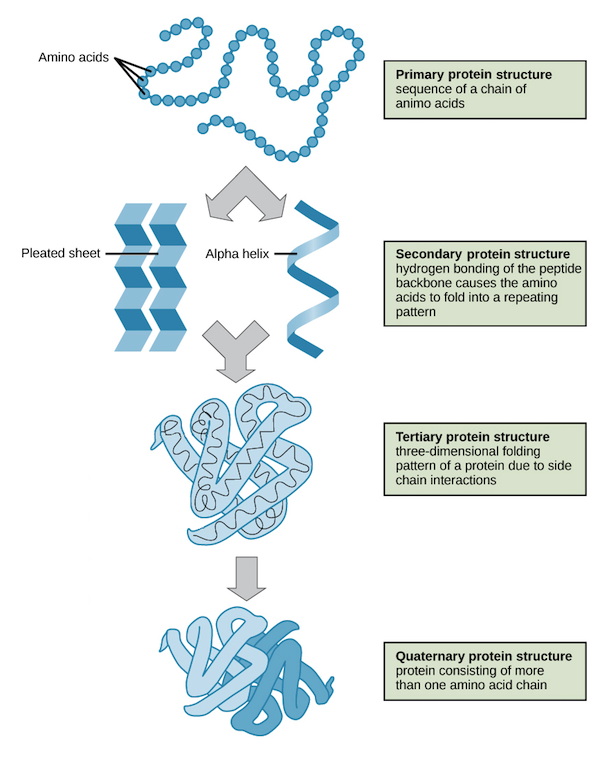
\includegraphics[width=0.5\textwidth]{"/Users/enrico/PROTEINS/tesi/immagini_tesi_ingelse/71225d815cafcc09102504abdf4e10927283be98.png"}
    \caption{Seocndaria}
\end{figure}



\section{Protein structure}
The scructure of the protein is important because it determines its function. 
The structure of a protein is divided into four levels:
\subsection{Primary Structure}
The primary structure refers to the linear sequence of amino acids in a protein chain, held together by peptide bonds. This sequence is unique for each protein and dictates the higher levels of structure.

\subsection{Secondary Structure}
The secondary structure refers to the local folding of the protein chain into regular patterns such as alpha-helices and beta-pleated sheets. These structures are stabilized by hydrogen bonds between the backbone atoms of the amino acids.

\subsection{Tertiary Structure}
The tertiary structure describes the three-dimensional folding of the entire protein molecule, including all its side chains. This level of structure is stabilized by interactions such as hydrogen bonds, ionic bonds, hydrophobic interactions, and disulfide bridges.

\subsection{Quaternary Structure}
The quaternary structure applies to proteins that consist of more than one polypeptide chain. It describes how these chains are arranged and interact with each other to form the functional protein complex.
\begin{figure}[H]
    \centering
    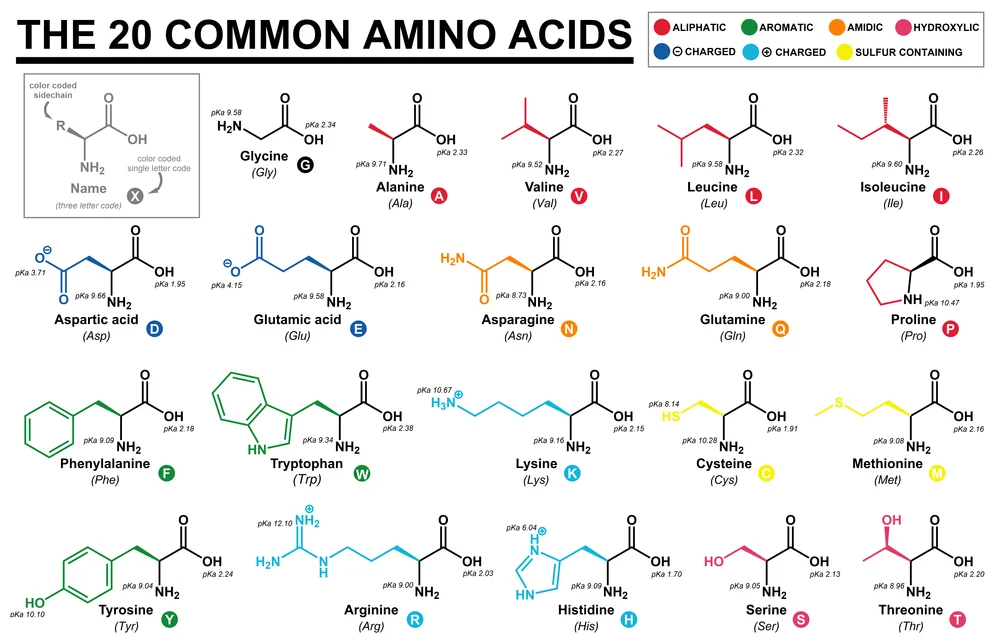
\includegraphics[width=0.5\textwidth]{/Users/enrico/PROTEINS/tesi/immagini_tesi_ingelse/ammino.png}
    \caption{Seocndaria}
\end{figure}

This structure are due to the interactions between the amino acids that compose the protein. 
Following we will see our model for the interaction between the amino acids.

\section{Allostericity}
Allostericity is the phenomen of the change of the protein structure by the trasmission of a signal from one site to another.
This avoid the protein to do various tasks in a regulated way.
Allostericity, from the Greek \textit{allos} (other) and \textit{stereos} (structure), refers to a phenomenon in which the interaction of a molecule (effector) with a specific site of a protein, known as the allosteric site, induces a conformational change that influences the functional activity of another site, usually the active site. This process does not occur through direct interactions between the two sites but rather via changes in the network of intramolecular interactions that regulate the structure and dynamics of the protein.

From a thermodynamic perspective, allostericity can be described as a modulation of the distribution of a protein's energy microstates. In other words, the interaction with an allosteric effector alters the set of available conformational states, facilitating or inhibiting access to functional configurations.

Mathematically, the phenomenon can be represented as a variation in the population of microstates \(\{s_i\}\), described by a weighted Boltzmann distribution:

\[
P(s_i) = \frac{e^{-\Delta F(s_i)/k_BT}}{\sum_j e^{-\Delta F(s_j)/k_BT}}
\]

where \(\Delta F(s_i)\) represents the free energy associated with microstate \(s_i\), \(k_B\) is the Boltzmann constant, and \(T\) is the absolute temperature.

The allosteric effect can also be quantified by considering the change in free energy associated with the effector interaction. For a protein with two principal states, \(R\) (relaxed) and \(T\) (tense), the allosteric equilibrium can be expressed in terms of an equilibrium constant:

\[
L = \frac{[T]}{[R]}
\]

where \([T]\) and \([R]\) represent the relative concentrations of the two conformational states. The presence of an effector modifies \(L\), stabilizing one state over the other.



Proteins are not rigid structures; instead, they are ensembles of conformational states that fluctuate over temporal and spatial scales. Allosteric effectors influence this dynamic network, remodeling energy pathways and connecting various functional states. Proteins can be represented as an ensemble of conformational states \(\{C_i\}\), where \(i\) denotes a specific conformational state. The distribution of populations across states is described by a partition function \(Z = \sum_i e^{-\beta E_i}\), where \(E_i\) is the energy associated with state \(C_i\) and \(\beta = \frac{1}{k_B T}\) is the thermodynamic factor.

An allosteric effector can be represented as a perturbation that modifies the energy landscape of the conformational states \(\{E_i\}\), remodeling energy pathways and altering the probability \(P_i\) of each state, where:

\[
P_i = \frac{e^{-\beta E_i}}{Z}, \quad \text{with } Z = \sum_i e^{-\beta E_i}.
\]

\begin{figure}[h]
    \centering
    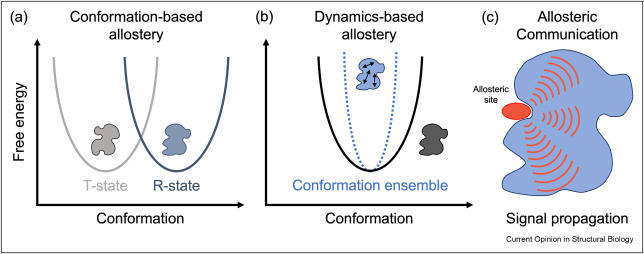
\includegraphics[width=\textwidth]{/Users/enrico/PROTEINS/tesi/immagini_tesi_ingelse/1-s2.0-S0959440X23002117-gr1.jpg}
    \caption{Schematic representation of allostericity: the interaction with an allosteric effector (site A) induces a conformational change that affects a distant site (site B).}
    \label{fig:allostericity_dynamics}
\end{figure}

This dynamic view integrates well with computational approaches such as molecular dynamics and interaction residue networks, which allow for the identification of specific pathways through which allosteric information propagates within the protein.

Understanding how and why the proteins fold into a functional structure it is useful for the study of the molecular basis of life and for the development of new drugs.
To study it we need to understand the causal mechanism and the propagation of the signal between the amino acids that compose the protein.
\section{Example of Allostericity in Hemoglobin and Red Blood Cells for Oxygen Transport}

Hemoglobin, the oxygen-transporting protein within red blood cells, is a classic example of an allosteric protein. Its function is to bind oxygen in the lungs and release it efficiently in tissues where oxygen is needed. This process is regulated by its allosteric properties, which involve conformational changes and cooperative binding.

\subsection{Mechanism of Allostericity in Hemoglobin}
Hemoglobin exists in two main states:
\begin{itemize}
    \item \textbf{T-state (Tense):} This state has a lower affinity for oxygen and is stabilized in tissues where oxygen levels are low.
    \item \textbf{R-state (Relaxed):} This state has a higher affinity for oxygen and is stabilized in the oxygen-rich environment of the lungs.
\end{itemize}

When the first oxygen molecule binds to one of hemoglobin's four subunits, it induces a conformational change that increases the affinity of the remaining subunits for oxygen. This phenomenon is called \textit{cooperative binding} and is a hallmark of allosteric regulation.

Similarly, the release of oxygen in tissues is facilitated by other effectors, such as:
\begin{itemize}
    \item \textbf{Carbon dioxide (\(CO_2\))} and \textbf{protons (\(H^+\))}, which stabilize the T-state (Bohr effect).
    \item \textbf{2,3-Bisphosphoglycerate (2,3-BPG)}, which reduces oxygen affinity to promote oxygen release in tissues.
\end{itemize}

\subsection{Practical Applications of Understanding Allostericity}
The study of allostericity in proteins, particularly hemoglobin, has several practical applications, including:

\begin{itemize}
    \item \textbf{Medical Interventions:} Developing drugs to modulate hemoglobin’s oxygen affinity could help treat conditions like sickle cell anemia, anemia, or hypoxia in high-altitude environments.
    \item \textbf{Artificial Blood Substitutes:} Designing synthetic hemoglobin mimics with tunable oxygen-binding properties for use in emergencies or surgeries.
    \item \textbf{Diagnostics:} Allosteric changes in hemoglobin can serve as biomarkers for detecting diseases such as diabetes (glycated hemoglobin levels) or metabolic disorders.
    \item \textbf{Enhanced Oxygen Delivery:} Creating treatments to improve oxygen delivery to tissues, potentially benefiting athletes or individuals with cardiovascular or pulmonary diseases.
\end{itemize}

\subsection{Summary of Potential Applications}
\begin{center}
    \begin{tabular}{|l|p{10cm}|}
        \hline
        \textbf{Application} & \textbf{Description} \\ \hline
        Medical Interventions & Drugs to adjust oxygen affinity in diseases like anemia or sickle cell anemia. \\ \hline
        Artificial Blood Substitutes & Synthetic hemoglobin for transfusions in emergencies. \\ \hline
        Biomarkers & Using hemoglobin changes to detect diseases like diabetes. \\ \hline
        Enhanced Oxygen Delivery & Improving oxygen transport for athletes or patients with breathing issues. \\ \hline
    \end{tabular}
\end{center}

Understanding the principles of allostericity allows researchers to develop novel strategies to improve human health and tackle diseases more effectively.
\chapter{PDZ Domain}

\section*{Definition of Protein Domains and the PDZ Domain}

In molecular biology, a \textbf{domain} is a specific region of a protein that can perform a structural or functional role independently from the rest of the protein. Domains are essential because they serve as modular units that recur and combine to form complex proteins with distinct functions.

\subsection*{Definition of Domain}
A protein domain is:
\begin{enumerate}
    \item \textbf{A structurally independent unit}: It is a portion of the protein that can fold into a stable three-dimensional structure on its own.
    \item \textbf{A functionally independent unit}: It can perform specific tasks, such as binding to a molecule or interacting with other proteins.
    \item \textbf{An evolutionary modular unit}: Domains are often reused in different proteins during evolution, allowing for the development of new functions.
\end{enumerate}

\subsection*{The PDZ Domain}
The \textbf{PDZ domain} is an example of a protein domain. The name "PDZ" is derived from the three proteins in which it was first identified:
\begin{itemize}
    \item \textbf{P}SD-95 (Protein Discs Large 4),
    \item \textbf{D}lgA (Drosophila discs large protein),
    \item \textbf{Z}O-1 (Zona Occludens 1).
\end{itemize}

\subsubsection*{Characteristics of the PDZ Domain}
\begin{itemize}
    \item \textbf{Length}: Typically consists of 80--90 amino acids.
    \item \textbf{Main Function}: Facilitates protein-protein interactions by recognizing specific peptide sequences, often located at the C-terminal region of other proteins.
    \item \textbf{Biological Role}:
    \begin{itemize}
        \item Assembling protein complexes at cellular membranes.
        \item Cellular signaling.
        \item Maintaining cell polarity.
    \end{itemize}
    \item \textbf{Structure}: The PDZ domain has a characteristic structure composed of an antiparallel beta-sheet and two alpha-helices.
\end{itemize}

\subsubsection*{Biological Importance}
The PDZ domain is essential for:
\begin{itemize}
    \item The assembly of multiprotein complexes, such as those involved in signal transduction.
    \item Proper spatial localization of proteins, for instance, in neuronal synapses.
    \item Maintaining membrane integrity and intercellular communication.
\end{itemize}


\chapter{Modelization of the Interaction between Amino Acids: GNM}
It's clear that the interactions between the amino acids that compose the protein are crucial for the folding of the protein into a functional structure.
So we need an hamiltonian to describe the system.
If the protein is at the equilibrium i will expect that the hamiltonian is a function of a potential which depends from the position every atom that constituted the PDZ specific domain.
So my hamiltonian $H$ will be \( H = V(\mathbf{r}) \), where \( \mathbf{r} \) is the vector that contains the position of every atom that constitute the protein.
Because this is a complex system we can't solve the problem exactly, so we need to use an approximation.

The second-order approximation of a function \( V(\mathbf{r}) \), around an equilibrium point \( \mathbf{r}_0 \), can be written as:

\begin{equation}
V(\mathbf{r}) \approx V(\mathbf{r}_0) + \nabla V(\mathbf{r}_0)^\top (\mathbf{r} - \mathbf{r}_0) + \frac{1}{2} (\mathbf{r} - \mathbf{r}_0)^\top \mathbf{H_V} (\mathbf{r} - \mathbf{r}_0)
\end{equation}

Where:
\begin{itemize}
    \item \( V(\mathbf{r}_0) \) is the value of the function at the equilibrium point \( \mathbf{r}_0 \).
    \item \( \nabla V(\mathbf{r}_0) \) is the gradient of the function, defined as:
    \begin{equation}
    \nabla V(\mathbf{r}) = \frac{\partial V}{\partial \mathbf{r}} \bigg|_{\mathbf{r} = \mathbf{r}_0}
    \end{equation}
    which equals zero if \( \mathbf{r}_0 \) represents a minimum point, so the equilibrium position.
    \item \( \mathbf{H_V} \) is the \textbf{Hessian matrix} of \( V(\mathbf{r}) \), defined as:
    \begin{equation}
		\mathbf{H_V} = \frac{\partial^2 V}{\partial \mathbf{r}^2} \bigg|_{\mathbf{r} = \mathbf{r}_0}
    \end{equation}
    \[
    \mathbf{H} = \begin{bmatrix}
    \frac{\partial^2 V}{\partial x_1^2} & \frac{\partial^2 V}{\partial x_1 \partial x_2} & \cdots & \frac{\partial^2 V}{\partial x_1 \partial x_{3N}} \\
    \frac{\partial^2 V}{\partial x_2 \partial x_1} & \frac{\partial^2 V}{\partial x_2^2} & \cdots & \frac{\partial^2 V}{\partial x_2 \partial x_{3N}} \\
    \vdots & \vdots & \ddots & \vdots \\
    \frac{\partial^2 V}{\partial x_{3N} \partial x_1} & \frac{\partial^2 V}{\partial x_{3N} \partial x_2} & \cdots & \frac{\partial^2 V}{\partial x_{3N}^2}
    \end{bmatrix}.
    \]
    and it is a symmetric matrix that describes the curvature of \( V(\mathbf{r}) \) around \( \mathbf{r}_0 \).
\end{itemize}

It is important to note that the \textbf{Hessian matrix} \( \mathbf{H_V} \) should not be confused with the \textbf{Hamiltonian}, which represents the total energy of a system in terms of conjugate coordinates (positions and momenta).

So apart from the constants we can write the hamiltonian as:

\begin{equation}
	V(\mathbf{r}) \approx\frac{1}{2} (\mathbf{r} - \mathbf{r}_0)^\top \mathbf{H_V} (\mathbf{r} - \mathbf{r}_0) \label{1.1}
\end{equation}
For simplicity, we can consider only the \(\alpha\)-carbon atoms because:

\begin{itemize}
    \item The \(\alpha\)-carbon atoms form the backbone of the protein, which defines its overall structure and shape.
    \item The positions of \(\alpha\)-carbon atoms are sufficient to reconstruct the global three-dimensional conformation of the protein.
    \item Considering only the \(\alpha\)-carbons significantly reduces the complexity of the system, lowering the number of degrees of freedom and making calculations more computationally efficient.
    \item The dynamics of \(\alpha\)-carbons often capture the collective motions of the protein, which are crucial for understanding its function (e.g., domain movements, opening of active sites).
    \item Experimental techniques such as X-ray crystallography and NMR frequently provide high-resolution data specifically for \(\alpha\)-carbon atoms, which serve as reference points for modeling (See section ).
This model is overlall extendaible to all other atoms of the protein.
\section{Interpretion of the Taylor Expansion: The Gaussian Network Model}
I can interpretate equation \eqref{1.1} not only as hamiltonian of the armonic oscillator  (springs-system) but also like a Network Model where every \(\alpha\)-carbon atom is a node that interacts with others node.
\subsubsection{Definition of a Graph}
A graph \( G \) is a mathematical structure used to model pairwise relations between objects. It consists of a set of vertices \( V \) (also called nodes) and a set of edges \( E \), where each edge connects a pair of vertices. Formally, a graph is denoted as \( G = (V, E) \). Graphs can be directed or undirected, weighted or unweighted, depending on the nature of the relationships they represent.

\begin{figure}[h]
    \centering
    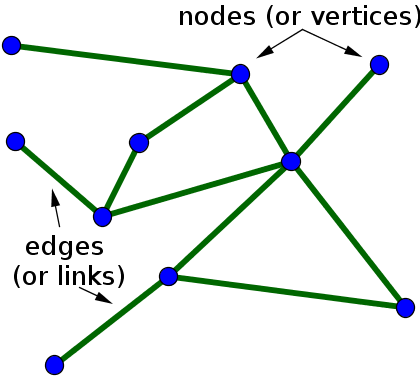
\includegraphics[width=\textwidth]{/Users/enrico/PROTEINS/tesi/immagini_tesi_ingelse/small_undirected_network_labeled-2.png}    
    \caption{Schematic representation of a Network.}
    \label{fig:Network}
\end{figure}
\subsubsection{Kirchhoff Matrix (Laplacian Matrix)}
The Kirchhoff matrix, also known as the graph Laplacian, is a matrix representation of a graph that encodes information about its structure. For a graph \( G \) with \( n \) vertices, the Laplacian matrix \( L \) is defined as:

\[
L = D - A
\]

Where:
\begin{itemize}
    \item \( D \) is the degree matrix, a diagonal matrix where each diagonal element \( d_{ii} \) is the degree of vertex \( i \) (the number of edges connected to it).
    \item \( A \) is the adjacency matrix, where \( a_{ij} = 1 \) if there is an edge between vertices \( i \) and \( j \), and \( 0 \) otherwise.
\end{itemize}
\subsubsection{Properties of the Degree Matrix}
The degree matrix \( D \) has the following properties:
\begin{itemize}
    \item \textbf{Diagonal Matrix:} \( D \) is diagonal, meaning all off-diagonal elements are zero.
    \item \textbf{Non-Negative Entries:} Each diagonal element \( d_{ii} \) represents the degree of vertex \( i \), which is always non-negative.
    \item \textbf{Relation to Graph Order:} For simple graphs, the sum of all diagonal elements of \( D \) equals twice the number of edges, i.e., \( \mathrm{trace}(D) = 2|E| \).
\end{itemize}

\subsubsection{Properties of the Adjacency Matrix}
The adjacency matrix \( A \) encodes the edge structure of the graph and has the following properties:
\begin{itemize}
    \item \textbf{Symmetry:} For undirected graphs, \( A \) is symmetric, i.e., \( a_{ij} = a_{ji} \).
    \item \textbf{Binary Entries:} For unweighted graphs, each element \( a_{ij} \in \{0, 1\} \), where \( 1 \) indicates the presence of an edge between \( i \) and \( j \), and \( 0 \) indicates absence.
    \item \textbf{Weighted Graphs:} For weighted graphs, \( a_{ij} \) takes the weight of the edge between vertices \( i \) and \( j \).
    \item \textbf{Self-Loops:} Diagonal entries \( a_{ii} \) indicate self-loops. For simple graphs, \( a_{ii} = 0 \).
    \item \textbf{Spectral Properties:} The eigenvalues of \( A \) provide insights into graph connectivity and other structural properties, such as bipartiteness and clustering.
\end{itemize}
\subsubsection{Mathematical Properties of the Network}
The graph Laplacian has several important mathematical properties:
\begin{itemize}
    \item \textbf{Symmetry:} For undirected graphs, \( L \) is symmetric and thus diagonalizable.
    \item \textbf{Positive Semi-definiteness:} The Laplacian matrix \( L \) is positive semi-definite, meaning that all its eigenvalues are non-negative.
    \item \textbf{Eigenvalues:} The smallest eigenvalue of \( L \) is always \( 0 \), corresponding to the eigenvector \( \mathbf{1} \) (a vector of all ones). The multiplicity of the zero eigenvalue indicates the number of connected components in the graph.
    \item \textbf{Combinatorial Interpretation:} The determinant of the reduced Laplacian matrix (obtained by removing one row and one column) gives the number of spanning trees in the graph.
\end{itemize}

\subsubsection{Inverse of Weighted Laplacian (Pseudo-Inverse)}
For a connected graph, the weighted Laplacian \( L \) is not invertible due to the zero eigenvalue. However, the Moore-Penrose pseudo-inverse \( L^+ \) can be computed. The pseudo-inverse is used in various applications such as electrical network analysis, random walks, and graph-based optimization. It satisfies:

\[
L^+ L = L L^+ = I - \frac{1}{n} \mathbf{1} \mathbf{1}^\top
\]

where \( n \) is the number of nodes and \( \mathbf{1} \) is a vector of all ones.
\subsection{Gaussian Network Model (GNM)}
For what we said before, now we can write the hamiltonian as:
\begin{equation}
    H(\mathbf{r}) \approx  \frac{1}{2} (\mathbf{r} - \mathbf{r}_0)^\top \mathbf{K} (\mathbf{r} - \mathbf{r}_0)
\end{equation}
Dove \( \mathbf{K} \) è la matrice laplaciana.
Per semplicità la scriveremo nel seguent modo:
\begin{equation}
    H(\mathbf{r}) \approx  \frac{1}{2} \mathbf{r}^\top \mathbf{K} \mathbf{r}
\end{equation}
o in componenti:
\begin{equation}
    H(\mathbf{r}) \approx  \frac{1}{2} \sum_{{i}_{j}} \mathbf{r_i} \mathbf{K_{i}_{j}} \mathbf{r_j}
\end{equation}
Dove $r$ è il vettore spostamente rispetto alla posizione di equilibrio di ciascun atomo.
Da questa modellizzazione del sistema seguono diverse proprietà e caratteristiche del sistema.
Initialy we can write the Probability density at the equilibrium as:
\begin{equation}
    P(\mathbf{r}) = \frac{1}{Z} e^{-\beta H(\mathbf{r})}
    \end{equation}
    \begin{equation}
    Z = \int e^{-\beta H(\mathbf{r})} \, d\mathbf{r}
    \end{equation}
At this point we can calculate the mean value of the position of the atoms:
\subsubsection{Mean Position}
The mean position \(\langle \bm{r} \rangle\) is given by:
\begin{equation}
\langle \bm{r} \rangle = \int \bm{r} P(\bm{r}) \, d\bm{r},
\end{equation}
where
\begin{equation}
P(\bm{r}) = \frac{1}{Z} e^{-\frac{\beta}{2} \bm{r}^\top \mathbf{K} \bm{r}},
\end{equation}
and the partition function is:
\begin{equation}
Z = \int e^{-\frac{\beta}{2} \bm{r}^\top \mathbf{K} \bm{r}} \, d\bm{r}.
\end{equation}

Substituting \(P(\bm{r})\) into the expression for \(\langle \bm{r} \rangle\), we have:
\begin{equation}
\langle \bm{r} \rangle = \frac{1}{Z} \int \bm{r} e^{-\frac{\beta}{2} \bm{r}^\top \mathbf{K} \bm{r}} \, d\bm{r}.
\end{equation}

The integrand \(\bm{r} e^{-\frac{\beta}{2} \bm{r}^\top \mathbf{K} \bm{r}}\) is symmetric with respect to \(\bm{r}\), and since there are no linear terms in the Hamiltonian, the Gaussian distribution is centered at \(\bm{r} = 0\). Therefore:
\begin{equation}
\langle \bm{r} \rangle = 0.
\end{equation}

\subsubsection{Covariance}
The covariance between \(r_i\) and \(r_j\) is given by:
\begin{equation}
\text{Cov}(r_i, r_j) = \langle r_i r_j \rangle - \langle r_i \rangle \langle r_j \rangle.
\end{equation}

Since \(\langle r_i \rangle = 0\), we have:
\begin{equation}
\text{Cov}(r_i, r_j) = \langle r_i r_j \rangle.
\end{equation}

Using the Boltzmann distribution:
\begin{equation}
P(\bm{r}) = \frac{1}{Z} e^{-\frac{\beta}{2} \bm{r}^\top \mathbf{K} \bm{r}},
\end{equation}
we compute:
\begin{equation}
\langle r_i r_j \rangle = \frac{1}{Z} \int r_i r_j e^{-\frac{\beta}{2} \bm{r}^\top \mathbf{K} \bm{r}} \, d\bm{r}.
\end{equation}

For a Gaussian distribution, the covariance matrix is:
\begin{equation}
\bm{\Sigma} = \beta^{-1} \mathbf{K}^{-1},
\end{equation}
where \((\mathbf{K}^{-1})_{ij}\) is the \((i,j)\)-th element of \(\mathbf{K}^{-1}\). Therefore:
\begin{equation}
\text{Cov}(r_i, r_j) = \frac{1}{\beta} (\mathbf{K}^{-1})_{ij}.
\end{equation}

\subsection*{Derivation of Diffraction Intensity with Atomic Vibrations}
The diffraction intensity in crystallography is influenced by the atomic vibrations around their mean positions. These vibrations are characterized by the mean squared displacement, denoted as $\langle u^2 \rangle$. To derive the expression for intensity, we start with the electron density modulated by atomic displacement.

Let the position of an atom be $\mathbf{r}$, with its displacement modeled as a Gaussian distribution around its mean position $\mathbf{r_0}$. The thermal motion leads to a modification of the scattering factor:
\[
f(\mathbf{q}) = f_0(\mathbf{q}) \cdot e^{-2\pi i \mathbf{q} \cdot \mathbf{u}}
\]
where:
\begin{itemize}
    \item $f_0(\mathbf{q})$: scattering factor for a stationary atom,
    \item $\mathbf{q}$: scattering vector,
    \item $\mathbf{u}$: displacement from the mean position.
\end{itemize}

The observed intensity $I(\mathbf{q})$ is proportional to the squared magnitude of the structure factor $F(\mathbf{q})$:
\[
I(\mathbf{q}) \propto |F(\mathbf{q})|^2,
\]
where $F(\mathbf{q})$ is the sum over all atomic contributions:
\[
F(\mathbf{q}) = \sum_j f_j(\mathbf{q}) e^{2\pi i \mathbf{q} \cdot \mathbf{r}_j}.
\]

Now consider the thermal vibrations. Averaging over the Gaussian distribution of displacements yields a damping factor:
\[
\langle e^{-2\pi i \mathbf{q} \cdot \mathbf{u}} \rangle = e^{-2\pi^2 \langle (\mathbf{q} \cdot \mathbf{u})^2 \rangle}.
\]
Assuming isotropic vibrations, this simplifies to:
\[
\langle (\mathbf{q} \cdot \mathbf{u})^2 \rangle = |\mathbf{q}|^2 \langle u^2 \rangle,
\]
where $\langle u^2 \rangle$ is the mean squared displacement. Substituting this back, the intensity is:
\[
I(\mathbf{q}) \propto |F(\mathbf{q})|^2 e^{-8\pi^2 \langle u^2 \rangle |\mathbf{q}|^2}.
\]

The factor $B = 8\pi^2 \langle u^2 \rangle$ emerges naturally, leading to:
\[
I(\mathbf{q}) \propto |F(\mathbf{q})|^2 e^{-B |\mathbf{q}|^2}.
\]

\subsection*{Importance of the Beta Factor as a Metric of Model Accuracy}
The beta factor ($B$) is a crucial metric in crystallographic modeling for several reasons:

\subsubsection*{1. Representation of Atomic Dynamics}
The beta factor reflects the thermal vibrations and dynamic behavior of atoms within the crystal. High $B$ values indicate greater atomic mobility or disorder, while low $B$ values suggest rigidity.

\subsubsection*{2. Assessment of Structural Flexibility}
Regions with elevated beta factors often correspond to flexible or disordered parts of the molecule, such as loops, termini, or unstructured regions. These provide insights into the functional dynamics of the macromolecule.

\subsubsection*{3. Indicator of Model Quality}
Unrealistically high or low beta factors across the structure can indicate modeling errors or issues with data quality, such as:
\begin{itemize}
    \item Poor resolution of the diffraction data.
    \item Incorrect assignment of atomic positions.
    \item Misrepresentation of isotropic vs. anisotropic motion.
\end{itemize}

\subsubsection*{4. Validation of Refinement}
During model refinement, the beta factors are optimized to fit the experimental data. If the refinement process yields consistent and reasonable beta factors, it supports the accuracy of the atomic model.

\subsubsection*{Conclusion}
The beta factor ($B$) serves as both a physical descriptor of atomic motion and a diagnostic tool for evaluating the quality of crystallographic models. Monitoring $B$ values provides insights into the structure's flexibility and ensures that the model faithfully represents the experimental data.

\section*{Model Evaluation: \(R^2\) and MAE}

\subsection*{\(R^2\): Coefficient of Determination}
The formula for \(R^2\) is:
\[
R^2 = 1 - \frac{\sum_{i=1}^n (y_i - \hat{y}_i)^2}{\sum_{i=1}^n (y_i - \bar{y})^2}
\]
Where:
\begin{itemize}
    \item \(y_i\): observed values,
    \item \(\hat{y}_i\): predicted values,
    \item \(\bar{y}\): mean of the observed values,
    \item \(n\): total number of data points.
\end{itemize}

\subsection*{MAE: Mean Absolute Error}
The formula for MAE is:
\[
\text{MAE} = \frac{1}{n} \sum_{i=1}^n |y_i - \hat{y}_i|
\]
Where:
\begin{itemize}
    \item \(y_i\): observed values,
    \item \(\hat{y}_i\): predicted values,
    \item \(n\): total number of data points.
\end{itemize}

\subsection*{Evaluation of Beta Factors and Model Quality}
In crystallography, the Beta factors (\(B\)) are an important metric to assess the quality of a structural model. The value of \(B\) is given by:
\[
B = 8\pi^2 \langle u^2 \rangle = 8\pi^2 \frac{k_B T}{k_{\text{eff}}}
\]
Where:
\begin{itemize}
    \item \(\langle u^2 \rangle\): mean squared atomic displacement,
    \item \(k_B\): Boltzmann constant,
    \item \(T\): absolute temperature,
    \item \(k_{\text{eff}}\): effective spring constant (describing atomic rigidity).
\end{itemize}

\subsubsection*{Importance of Beta Factors in Model Quality}
1. **Thermal Motion Representation**:
    Beta factors capture the vibrational dynamics of atoms. Consistent \(B\) values across the model indicate reliable representation of the thermal motion.
    
2. **Detection of Disordered Regions**:
    High \(B\) values typically correspond to disordered or flexible regions in the structure (e.g., loops or termini).

3. **Model Refinement**:
    During refinement, fitting experimental data should yield realistic \(B\) values. Overly high or low \(B\) values may indicate incorrect atomic positions or errors in data processing.

4. **Outlier Detection**:
    A plot of \(B\) values versus residue number can reveal anomalies or poorly modeled regions in the structure.

\subsection*{Combining Metrics for Model Assessment}
To fully evaluate the quality of a model:
\begin{itemize}
    \item Use \(R^2\) or a similar metric to evaluate how well the predicted data fits the observed data (e.g., intensities in crystallography).
    \item Use MAE or RMSD to assess the absolute error between predictions and observations.
    \item Analyze \(B\) factors to validate structural consistency and detect regions of disorder or flexibility.
\end{itemize}







\subsection*{Conclusion}
Combining statistical measures such as \(R^2\) and MAE with physical metrics like Beta factors provides a comprehensive evaluation of the model's accuracy and reliability.

\section{Understanding and Causality of allosteric mechanisms in proteins}
The correlation not only avoid to test the quality of the model through the beta factors but also avoid to understand the interactions between nodes.
Our goal is to understand what is the allosteric site, that is the site from wich the signal is transmitted to the other sites of the protein. 
As it often said, correlation does not imply causation.
\begin{figure}[h]
    \centering
    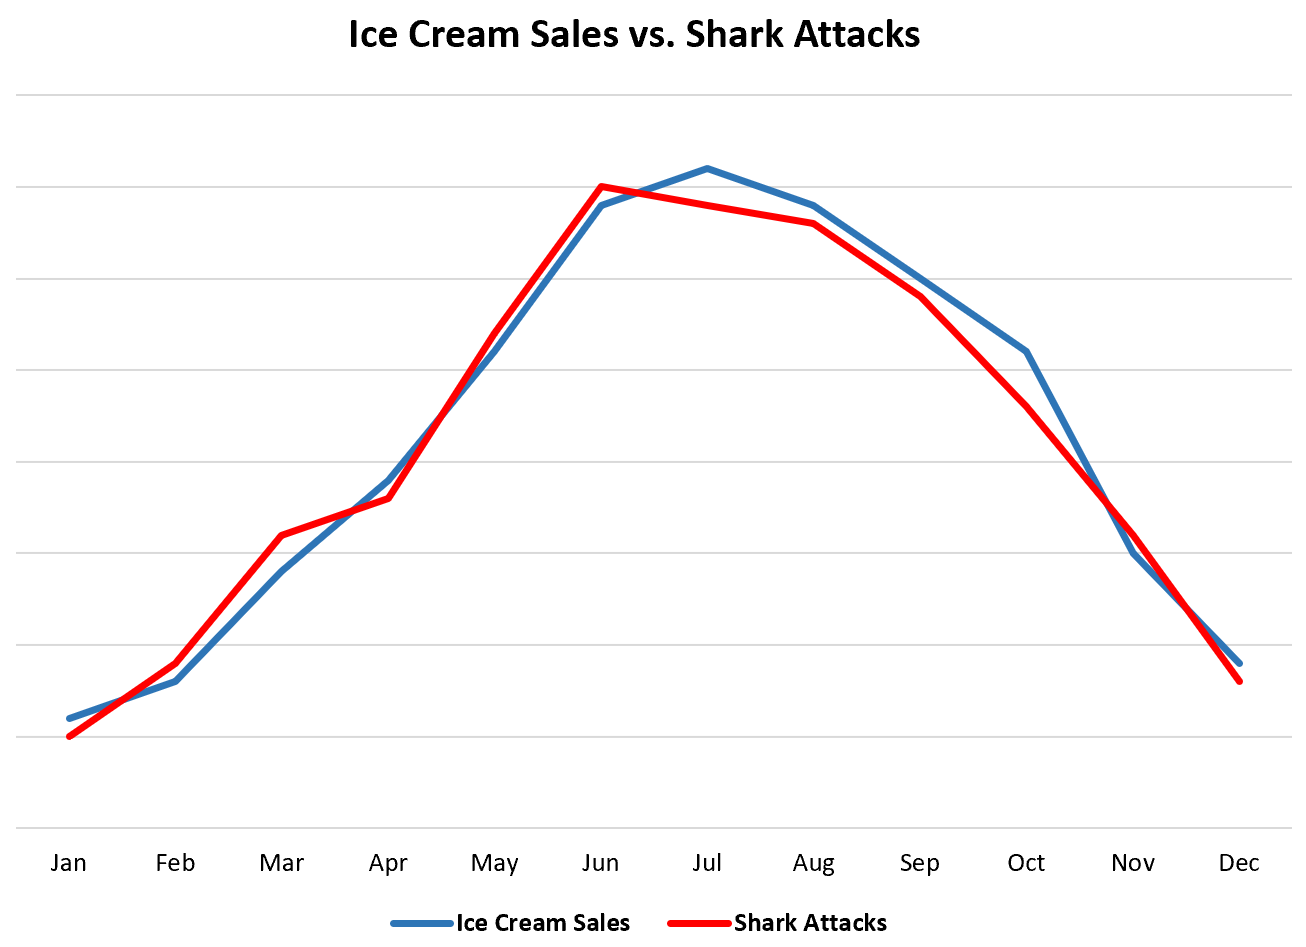
\includegraphics[width=\textwidth]{/Users/enrico/PROTEINS/tesi/immagini_tesi_ingelse/corrCause1.png}    
    \caption{Correlation is not causation.}
    \label{fig:Correlation is not causation}
\end{figure}
Causality refers to the relationship between causes and effects, where one event (the cause) directly influences or produces another event (the effect). Formally, causality can be defined as follows:

\begin{quote}
    A phenomenon \( A \) is said to be the cause of phenomenon \( B \) if the occurrence or change in \( A \) leads to a corresponding occurrence or change in \( B \), provided that all other conditions remain constant.
\end{quote}

Causality is a foundational concept in various fields, including physics, philosophy, and statistics. It implies a directional influence, where the cause precedes the effect in time and is necessary, sufficient, or contributory for the effect to occur. 

In mathematical terms, causal relationships can often be expressed using models such as:

\[
B = f(A, \text{other factors}) 
\]

where \( f \) is a functional relationship capturing how \( A \) and other factors jointly determine \( B \). In experimental contexts, causality is typically established through controlled interventions and the observation of corresponding changes.
\section*{Deterministic and Stochastic Causality}

Causality can be broadly classified into two types: deterministic and stochastic. In \textbf{deterministic causality}, a specific cause invariably leads to a specific effect. Mathematically, if an event \( A \) causes an event \( B \), then \( B \) will always occur whenever \( A \) occurs. This relationship can be represented as \( A \implies B \), meaning that \( A \) is both necessary and sufficient for \( B \). Deterministic causality is commonly observed in systems governed by precise physical laws, such as the equations of motion in classical mechanics, where given initial conditions and forces, the trajectory of an object is entirely predictable.

In contrast, \textbf{stochastic causality} acknowledges that many causal relationships are probabilistic rather than absolute. Here, the occurrence of \( A \) increases the likelihood of \( B \), but \( B \) does not necessarily follow \( A \). This can be expressed probabilistically as \( P(B|A) > P(B|\neg A) \), indicating that \( A \) raises the probability of \( B \). Stochastic causality is particularly prevalent in complex systems, such as biology or social sciences, where multiple factors interact, and outcomes are influenced by inherent randomness or uncertainty. For example, smoking increases the probability of lung cancer, but not all smokers develop cancer.

Both deterministic and stochastic causality play crucial roles in understanding natural phenomena. While deterministic causality provides precise predictive power, stochastic causality is essential for modeling systems where randomness and variability are inherent. Together, these concepts offer a comprehensive framework for analyzing causal relationships across disciplines.

\section*{Geometric Perspective of Causality and Shannon Entropy}
When all dimensions or variables of the system are fully known, the uncertainty about future states vanishes, and the system transitions into a deterministic regime.

This idea can be linked to Shannon entropy, defined as:
\[
H(X) = -\sum_{i} P(x_i) \log P(x_i),
\]
where \( X \) is a random variable with possible states \( x_i \) and \( P(x_i) \) is the probability of \( x_i \). When \( H(X) = 0 \), the system has no uncertainty, indicating complete predictability of the state \( X \).

In a deterministic system, knowing all dimensions eliminates ambiguity, allowing the precise prediction of future states. However, in practice:
\begin{itemize}
    \item Complex systems often exhibit chaotic or stochastic behavior, making predictions challenging even if the system is deterministic.
    \item Non-linear dynamics can amplify small uncertainties, leading to an apparent increase in unpredictability.
\end{itemize}

Thus, while \( H(X) = 0 \) implies determinism in theory, practical limitations and system complexities must be considered in real-world applications.

To understand the causality of allosteric mechanisms in proteins, we need to investigate the underlying physical interactions and pathways that transmit signals between distant sites.
For theses reasons we need also another indicators:
\subsection{Rensponse Function}
\section*{Linear Response Theorem (Positions)}

The linear response theorem, expressed in terms of the positions \(\mathbf{r}_i\), describes how the average position of a particle \(i\) responds to a perturbation applied to parameter \(j\). The response is given by:

\[
R_{ij} = \frac{\partial \langle \mathbf{r}_i \rangle}{\partial f_j}
\]

Where:
- \(\mathbf{r}_i\) is the position of particle \(i\) relative to its equilibrium position.
- \(f_j\) is an external force applied to particle \(j\).
- \(\langle \mathbf{r}_i \rangle\) is the average position of particle \(i\).

\subsection*{Relation to Correlations}

The response can also be expressed in terms of the correlations between the fluctuations in the positions of particles \(i\) and \(j\):

\[
R_{ij} = \beta \langle \delta \mathbf{r}_i \cdot \delta \mathbf{r}_j \rangle
\]

Where:
- \(\delta \mathbf{r}_i = \mathbf{r}_i - \langle \mathbf{r}_i \rangle\) is the fluctuation of the position from its average value.
- \(\beta = \frac{1}{k_B T}\) is the inverse thermal energy, with \(k_B\) being the Boltzmann constant and \(T\) the temperature.
- \(\langle \delta \mathbf{r}_i \cdot \delta \mathbf{r}_j \rangle\) is the scalar product of the fluctuations in the positions of particles.

\subsection*{Physical Interpretation}

This result states that the linear response of the system to a perturbation is proportional to the thermal correlation between the fluctuations of the particles' positions. It reflects the connection between the equilibrium properties of the system and its dynamic response.

\subsection*{Why is Linear Response an Indicator of Causality?}

The linear response \(R_{ij}\) can be interpreted as an indicator of causality because it measures the direct influence of a change in parameter \(j\) (e.g., an external force) on variable \(i\) (e.g., position, velocity, or another observable). This connection arises for the following reasons:

\begin{itemize}
    \item \textbf{Direct cause-effect relationship:} The response \(R_{ij}\) explicitly quantifies how a perturbation \(f_j\) applied to \(j\) influences the behavior of \(i\). This reflects causality since the perturbation precedes the response.
    \item \textbf{Asymmetry of the response:} Causality implies asymmetry: if \(j\) causes a change in \(i\), the reverse (i.e., \(i\) influencing \(j\)) does not necessarily occur. In the linear response framework, \(R_{ij}\) specifically measures the influence of \(j\) on \(i\).
    \item \textbf{Relation to equilibrium correlations:} The proportionality \(R_{ij} = \beta \langle \delta \mathbf{r}_i \cdot \delta \mathbf{r}_j \rangle\) implies that the equilibrium correlations encode information about the system's ability to propagate changes. This reinforces the causal interpretation.
\end{itemize}

In summary, the linear response is a quantitative framework to understand how perturbations propagate through a system, reflecting causal influences between different components.
\section*{Transfer Entropy: Formula, Proof, and Causality}

\subsection*{Definition of Transfer Entropy}
The \textit{Transfer Entropy} (TE) measures the directional flow of information from a source variable \(x_j\) to a target variable \(x_i\). It quantifies how much the knowledge of past states of \(x_j\) improves the prediction of future states of \(x_i\), beyond what is already provided by the past states of \(x_i\) itself. The TE is defined as:

\[
TE_{j \to i}(t) = H[x_i(t + \tau) \mid x_i(\tau)] - H[x_i(t + \tau) \mid x_i(\tau), x_j(\tau)]
\]

Where:
\begin{itemize}
    \item \(H[a \mid b]\): Conditional Shannon entropy of variable \(a\) given \(b\).
    \item \(x_i(t + \tau)\): State of \(x_i\) at time \(t + \tau\).
    \item \(x_i(\tau), x_j(\tau)\): States of \(x_i\) and \(x_j\) at time \(\tau\).
\end{itemize}

\subsection*{Transfer Entropy for Gaussian Systems}
For stationary Gaussian processes, the Transfer Entropy can be computed analytically. Using the covariance matrices of the processes, the TE is given by:

\[
TE_{j \to i}(t) = -\frac{1}{2} \ln \left(1 - \frac{\alpha_{ij}(t)}{\beta_{ij}(t)}\right)
\]

Where:
\[
\alpha_{ij}(t) = [C_{ii}(0)C_{ij}(t) - C_{ij}(0)C_{ii}(t)]^2
\]
\[
\beta_{ij}(t) = [C_{ii}(0)C_{jj}(0) - C_{ij}^2(0)][C_{ii}^2(0) - C_{ii}^2(t)]
\]

Here, \(C_{ij}(t)\) represents the time-lagged cross-correlation between variables \(x_i\) and \(x_j\), while \(C_{ii}(0)\) and \(C_{jj}(0)\) are the variances of \(x_i\) and \(x_j\), respectively.

\subsection*{Proof Sketch for Gaussian TE}
The derivation relies on the Gaussian property that conditional entropies can be expressed in terms of covariance matrices. For a system described by variables \(x_i(t)\), \(x_i(0)\), and \(x_j(0)\), the covariance matrix is:

\[
\Omega = \begin{bmatrix}
C_{ii}(0) & C_{ii}(t) & C_{ij}(t) \\
C_{ii}(t) & C_{ii}(0) & C_{ij}(0) \\
C_{ij}(t) & C_{ij}(0) & C_{jj}(0)
\end{bmatrix}
\]

The conditional covariance matrices are computed to find \(TE_{j \to i}\) based on the definition of conditional entropy. After algebraic manipulation, the formula for Gaussian TE above is obtained.

\subsection*{Causality and Transfer Entropy}
Transfer Entropy is a powerful indicator of causality for the following reasons:
\begin{itemize}
    \item \textbf{Directionality:} TE is asymmetric (\(TE_{j \to i} \neq TE_{i \to j}\)), capturing the directional flow of information from \(x_j\) to \(x_i\).
    \item \textbf{Temporal dependence:} By using time-lagged variables, TE inherently respects the time ordering required for causation.
    \item \textbf{Beyond correlation:} While correlations measure symmetric associations, TE specifically quantifies the influence of one variable on another, conditioned on their histories.
\end{itemize}

\subsection*{Comparison with Correlation}
\begin{itemize}
    \item \textbf{Symmetry:} Correlation is symmetric (\(C_{ij} = C_{ji}\)), whereas TE is directional.
    \item \textbf{Causal inference:} Correlation measures only association, which can be spurious. TE identifies directed influences and distinguishes cause from effect.
    \item \textbf{Applications:} TE is particularly useful in systems with nonlinear dynamics, where correlations may fail to capture the true dependencies.
\end{itemize}






\chapter{Stochastic process}
By definition we can associate a stochastic process to a set of random variables that evolve over time. 
The evolution of the process is governed by probabilistic laws, and each random variable represents the state of the system at a specific time point. 
In general we have:
\begin{equation}
    \frac{dX_t}{dt} = -\nabla H(X_t) + \eta_t,
    \end{equation}
    
dove:
\begin{itemize}
    \item \( X_t \) rappresenta lo stato del sistema al tempo \( t \),
    \item \( H(X_t) \) è la Hamiltoniana del sistema, che governa la dinamica deterministica,
    \item \( -\nabla H(X_t) \) è il gradiente della Hamiltoniana (che fornisce la direzione di maggiore variazione),
    \item \( \eta_t \) è un termine di rumore stocastico (spesso modellato come un rumore bianco gaussiano con varianza \( \sigma^2 \)).
\end{itemize}
So for our specific hamiltonian we can write:
\begin{equation}
H(\mathbf{r}) \approx \frac{1}{2} \sum_{i,j} \mathbf{r}_i \mathbf{K}_{ij} \mathbf{r}_j,
\end{equation}

the gradient with respect to \(\mathbf{r}\) is given by:

\begin{equation}
\nabla H(\mathbf{r}) = \mathbf{K} \mathbf{r},
\end{equation}

where \(\mathbf{K}\) is the matrix of coefficients \(\mathbf{K}_{ij}\).

### Vectorial Form

The stochastic process dynamics in vectorial form are:

\begin{equation}
\frac{d\mathbf{r}_t}{dt} = -\mathbf{K} \mathbf{r}_t + \boldsymbol{\eta}_t,
\end{equation}

where:
\begin{itemize}
    \item \(\mathbf{r}_t\) is the state vector at time \(t\),
    \item \(-\mathbf{K} \mathbf{r}_t\) is the deterministic term derived from the Hamiltonian,
    \item \(\boldsymbol{\eta}_t\) is a stochastic noise vector (e.g., components are independent and Gaussian distributed).
\end{itemize}
In component form, the system is written as:
\begin{equation}
\frac{d\mathbf{r}_{i,t}}{dt} = -\sum_{j} \mathbf{K}_{ij} \mathbf{r}_{j,t} + \eta_{i,t},
\end{equation}

where:
\begin{itemize}
    \item \(i\) denotes the index of the vector component,
    \item \(\mathbf{K}_{ij}\) is the element of the matrix \(\mathbf{K}\),
    \item \(\mathbf{r}_{j,t}\) is the \(j\)-th component of the state vector at time \(t\),
    \item \(\eta_{i,t}\) is the noise term associated with the \(i\)-th component.
\end{itemize}

The analytical solution, assuming an initial condition \(\mathbf{r}_0\), is:

\begin{equation}
\mathbf{r}_t = e^{-\mathbf{K} t} \mathbf{r}_0 + \int_0^t e^{-\mathbf{K} (t-s)} \boldsymbol{\eta}_s \, ds.
\end{equation}

In this expression:
\begin{itemize}
    \item \(e^{-\mathbf{K} t}\) is the matrix exponential of \(-\mathbf{K} t\),
    \item The first term, \(e^{-\mathbf{K} t} \mathbf{r}_0\), represents the deterministic evolution,
    \item The second term, \(\int_0^t e^{-\mathbf{K} (t-s)} \boldsymbol{\eta}_s \, ds\), accounts for the stochastic contributions from the noise.
\end{itemize}

The solution combines deterministic decay driven by \(-\mathbf{K} \mathbf{r}_t\) and stochastic fluctuations due to \(\boldsymbol{\eta}_t\).

The correlation function is defined as:

\begin{equation}
\langle \mathbf{r}_t \mathbf{r}_\tau^\top \rangle.
\end{equation}

Substituting the solution and simplifying, we obtain:

\begin{equation}
\langle \mathbf{r}_t \mathbf{r}_\tau^\top \rangle = e^{-\mathbf{K} t} \langle \mathbf{r}_0 \mathbf{r}_0^\top \rangle e^{-\mathbf{K}^\top \tau}
+ \int_0^{\min(t, \tau)} e^{-\mathbf{K} (t-s)} \mathbf{Q} e^{-\mathbf{K}^\top (\tau-s)} \, ds.
\end{equation}

In this expression:
\begin{itemize}
    \item \(e^{-\mathbf{K} t}\) is the matrix exponential,
    \item \(\langle \mathbf{r}_0 \mathbf{r}_0^\top \rangle\) is the initial covariance matrix of \(\mathbf{r}_0\),
    \item \(\mathbf{Q}\) is the noise covariance matrix.
\end{itemize}



\section*{Response Function and Transfer Entropy}

### Response Function

The response function \(R_{ij}(t)\) is defined as:

\begin{equation}
R_{ij}(t) = \frac{C_{ij}(t)}{C_{ij}(0)},
\end{equation}

where the correlation \(C_{ij}(t)\) is given by the analytical solution:

\begin{equation}
C_{ij}(t) = \int_0^t \int_0^t e^{-\mathbf{K} (t-s)} \mathbf{Q} e^{-\mathbf{K}^\top (t-u)} \, ds \, du,
\end{equation}

and \(C_{ij}(0)\) is the initial correlation:

\begin{equation}
C_{ij}(0) = \langle \mathbf{r}_{i,0} \mathbf{r}_{j,0} \rangle.
\end{equation}

Thus, the response function becomes:

\begin{equation}
R_{ij}(t) = \frac{\int_0^t \int_0^t e^{-\mathbf{K} (t-s)} \mathbf{Q} e^{-\mathbf{K}^\top (t-u)} \, ds \, du}{C_{ij}(0)}.
\end{equation}

### Transfer Entropy

The transfer entropy \(TE_{j \to i}(t)\) is defined as:

\begin{equation}
TE_{j \to i}(t) = -\frac{1}{2} \ln \left(1 - \frac{\alpha_{ij}(t)}{\beta_{ij}(t)}\right),
\end{equation}

where:
\[
\alpha_{ij}(t) = \left[C_{ii}(0)C_{ij}(t) - C_{ij}(0)C_{ii}(t)\right]^2,
\]
\[
\beta_{ij}(t) = \left[C_{ii}(0)C_{jj}(0) - C_{ij}^2(0)\right]\left[C_{ii}^2(0) - C_{ii}^2(t)\right].
\]

#### Substituting Correlation Expressions

1. The diagonal correlations are:

\begin{equation}
C_{ii}(t) = \int_0^t \int_0^t e^{-\mathbf{K} (t-s)} \mathbf{Q}_{ii} e^{-\mathbf{K}^\top (t-u)} \, ds \, du.
\end{equation}

2. The off-diagonal correlations are:

\begin{equation}
C_{ij}(t) = \int_0^t \int_0^t e^{-\mathbf{K} (t-s)} \mathbf{Q}_{ij} e^{-\mathbf{K}^\top (t-u)} \, ds \, du.
\end{equation}

Substituting these into \(\alpha_{ij}(t)\) and \(\beta_{ij}(t)\):

\[
\alpha_{ij}(t) = \left[\langle \mathbf{r}_{i,0}^2 \rangle \cdot C_{ij}(t) - C_{ij}(0) \cdot C_{ii}(t)\right]^2,
\]

\[
\beta_{ij}(t) = \left[\langle \mathbf{r}_{i,0}^2 \rangle \langle \mathbf{r}_{j,0}^2 \rangle - C_{ij}^2(0)\right] \cdot \left[\langle \mathbf{r}_{i,0}^2 \rangle^2 - C_{ii}^2(t)\right].
\]

Finally, substituting these into the transfer entropy expression:

\begin{equation}
TE_{j \to i}(t) = -\frac{1}{2} \ln \left(1 - \frac{\left[\langle \mathbf{r}_{i,0}^2 \rangle \cdot C_{ij}(t) - C_{ij}(0) \cdot C_{ii}(t)\right]^2}{\left[\langle \mathbf{r}_{i,0}^2 \rangle \langle \mathbf{r}_{j,0}^2 \rangle - C_{ij}^2(0)\right] \cdot \left[\langle \mathbf{r}_{i,0}^2 \rangle^2 - C_{ii}^2(t)\right]}\right).
\end{equation}
\chapter{Conclusions}




\newpage
\null
\thispagestyle{empty}
\newpage

\begin{thebibliography}{10}
\bibitem{ref} NASA, \emph{"Dark Energy, Dark Matter"}.
\end{thebibliography}
\end{document}